%%%%%%%%%%%%%%%%%%%%%%%%%%%%%%%%%%%%%%%%%%%%%%%%%%%%%%%%%%%%%%%%%
%  _____       ______   ____									%
% |_   _|     |  ____|/ ____|  Institute of Embedded Systems	%
%   | |  _ __ | |__  | (___    Wireless Group					%
%   | | | '_ \|  __|  \___ \   Zuercher Hochschule Winterthur	%
%  _| |_| | | | |____ ____) |  (University of Applied Sciences)	%
% |_____|_| |_|______|_____/   8401 Winterthur, Switzerland		%
%																%
%%%%%%%%%%%%%%%%%%%%%%%%%%%%%%%%%%%%%%%%%%%%%%%%%%%%%%%%%%%%%%%%%

\chapter{Metastabilität}\label{chap.metastabilitat}

\section{Metastabiler Zustand}\label{sect.meatastabil_def}
Metastabilität bedeutet, dass der Ausgang eines Flip-Flops nicht dem Eingang entsprechen \textit{muss}. In einem metastabilen Zustand kann ein Ausgang korrekt sein, muss aber nicht.
Im Idealfall wählt wählt ein Flip-Flop seinen Ausgangswert selbst (siehe Abbildung \ref{fig.metastabil.schlimmster_Fal} oberes Signal). Im schlechten Fall “hängt” sich das Flip-Flop “auf” und toggelt permanent zwischen '0' und '1' (Abbildung \ref{fig.metastabil.schlimmster_Fal} unteres Signal).

\begin{figure}[H]
	\centering
	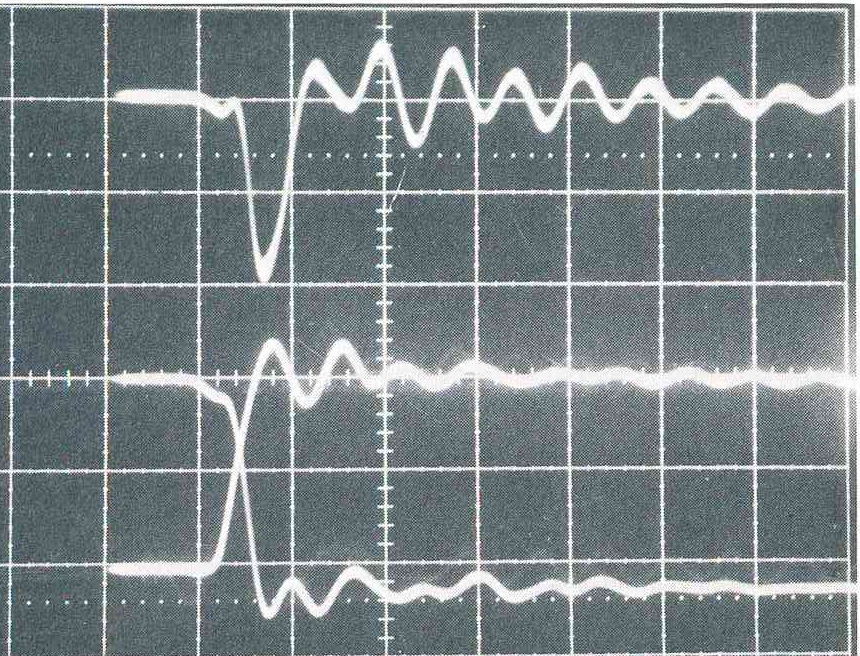
\includegraphics[width=0.4\textwidth]{images/metastability/metastability_2_IO.png}
	\caption{Metastabilität schlimmster Fall \cite{F_metastability}}
	\label{fig.metastabil.schlimmster_Fall}
\end{figure}


\section{Ursache von Metastabilität}\label{sect.meatastabil_ursache}

Die Ursache unsicherer Ausgangswerte liegen darin, dass das Inputsignal eines Flip-Flops zur falschen Zeit wechselt. \\
\newline
''If data inputs to a flip-flop are changing at the instant of the clock pulse, a problem known as \textit{metastability} may occur. In the metastable case, the flip-flop does not settle in to a stable state'' \cite{ReferenceManual} \\
\newline
''If the amplitude of the runt pulse is \textit{exactly the treshold level of the SET input of the output cell}, the cell will be driven to its metastable state. The metastable state is the condition that is roughly defined as ''half SET and half RESET'' \cite{F_metastability}\\
\newpage
Trifft der anzulegende Wert zu spät ein wird die \textit{setup time}) verletzt und wird der Signalwert zu früh entwendet, verletzt die \textit{hold time}). Metastabilität kann vermieden werden, wenn diese zwei Zeiten strikt eingehalten werden:\\
\newline
''Metastabilit is avoided by holding the information stable before and after the clock pulse  for a set period of time, called the setup time for the data line an the hold time for the control line.''\cite{ReferenceManual}
\begin{figure}[H]
	\centering
	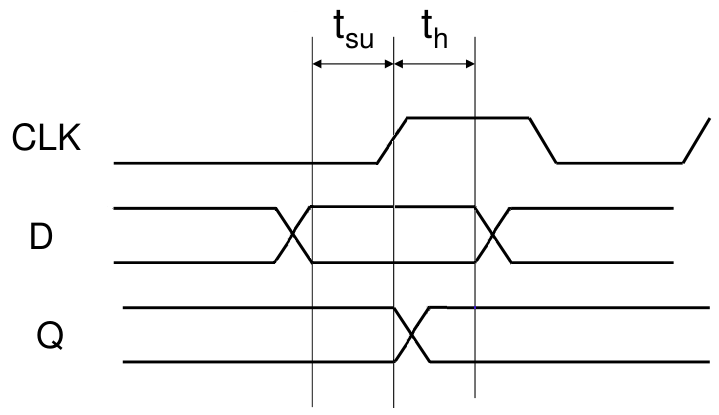
\includegraphics[width=0.4\textwidth]{images/metastability/kritscheZeit_FF.png}
	\caption{Einhalten der Datenzeiten}
	\label{fig.metastabil.kritisches_zeitfenster}
\end{figure}

Um Metastabilität zu vermeiden, sollte die Logik möglichst klein, die Bauteile beieinander und der Systemtakt an die längste Pfadzeit angepasst werden. Der maximal erlaubte Systemtakt kann in quartus mit dem Timequest Time Analyser abgefragt werden.\\


\section{Metastabilität erzeugen}\label{sect.meatastabil_erzeugen}

\subsection{Konzept}\label{sect.metastabil_ansatz}
Aufgebaut wird ein System mit zwei \textit{clock domains}. Eine \textit{clock domain}, Gebiet 1,  beinhaltet einen Zähler, der an das Gebiet 2 asynchrone Impulse sendet. Gebiet 2 verarbeitet diese Impulse in einer \textit{finate state machine}. Bei korrekter Funktionsweise wechset die \textit{fsm} zwischen den definierten \textit{states}. Funktioniert sie falsch, fällt die \textit{fsm} in einen \textit{state}, den sie nicht implementiert hat.\\

\begin{figure}[H]
	\centering
	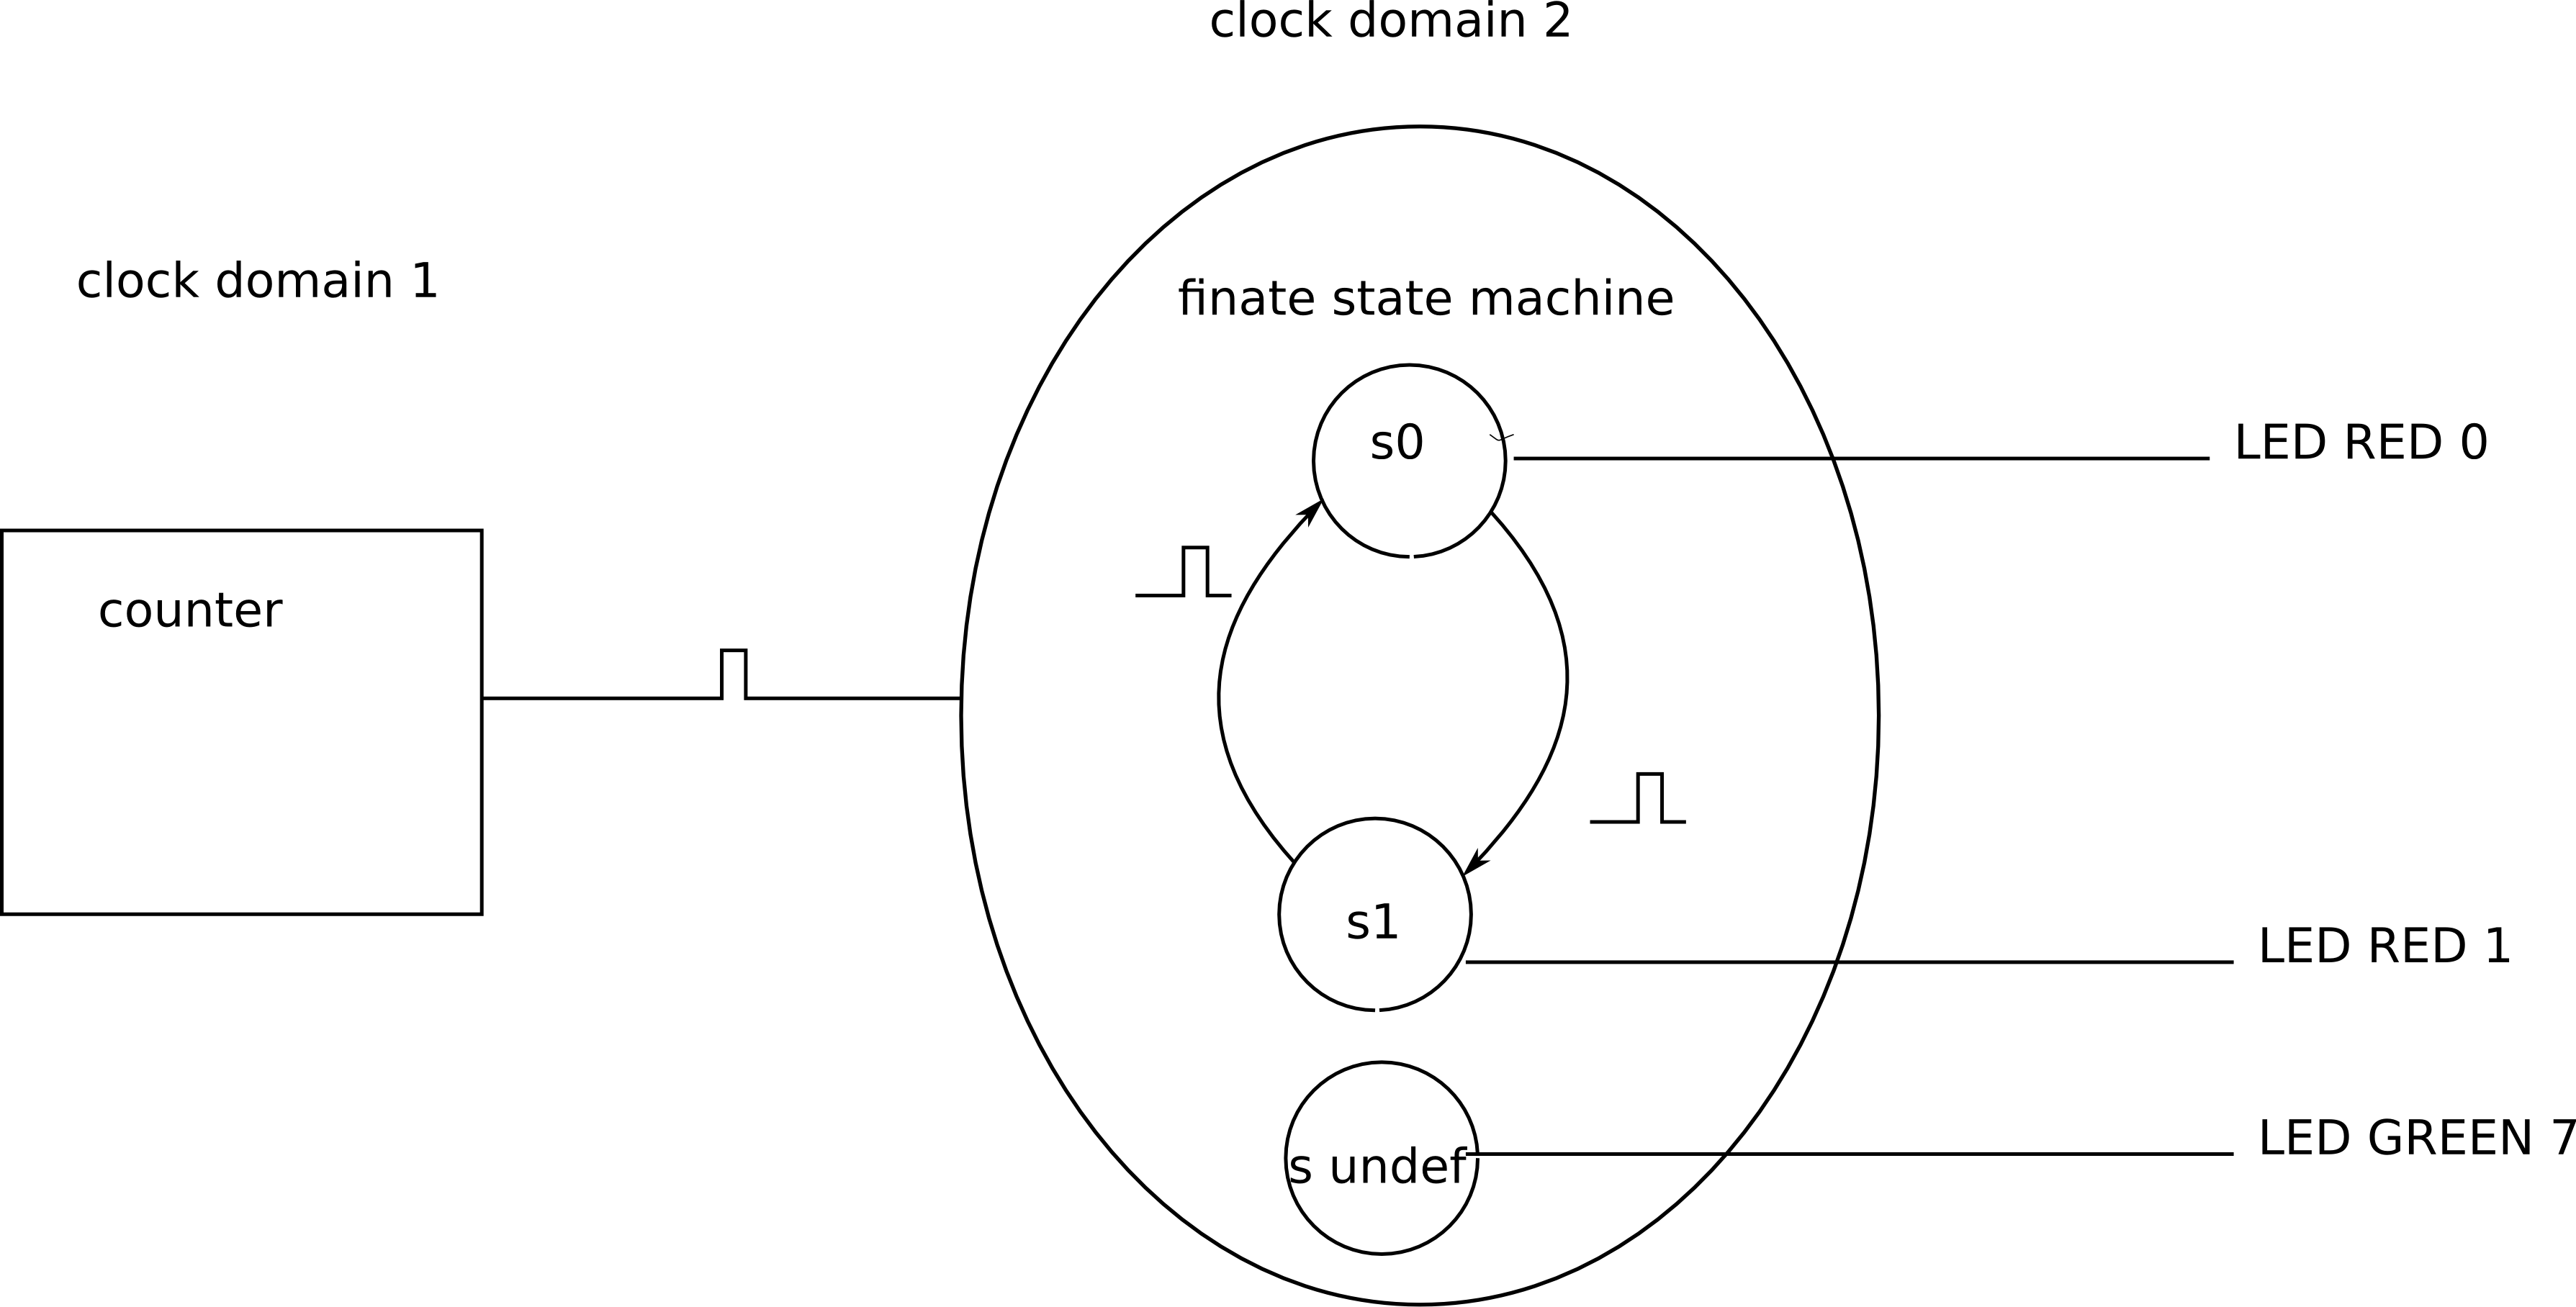
\includegraphics[width=0.8\textwidth]{images/metastability/konzept.png}
	\caption{Konzept Metastabilität nachweisen}
	\label{fig.metastabil.fsm}
\end{figure}


\subsection{Umsetzung}\label{sect.metastabil_implementation}
Als Hardware wird das altera development board De2 genommen und mit der Software quartus 13osp0 gearbeitet. Die die zwei Takte nicht Vielfache voneinander sein dürfen, wure für den Zähler ein Takt von 27 MHz und für die fsm ein Takt von 50 MHz. Der Takt des Zählers ist leicht schneller als die Hälfte der fsm und schiebt sich langsam vorwärts (siehe Abbildung \ref{fig.metastabil.takte}). Das Verletzen der \textit{setup time} ist somit nur eine Frage der Zeit.

\begin{figure}[H]
	\centering
	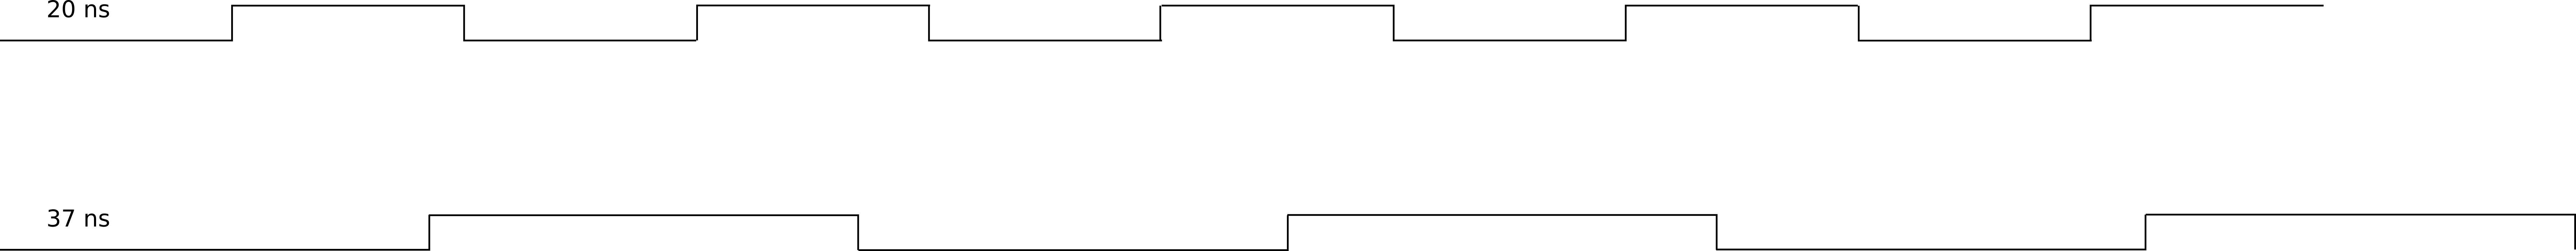
\includegraphics[width=0.8\textwidth]{images/metastability/2_takte.png}
	\caption{Die zwei Taktzeiten}
	\label{fig.metastabil.takte}
\end{figure}

Die Zustandsüberprüfung erfolgt über das Ausgaben des aktuellen Zustands auf den zwei roten LEDs. 
\begin{itemize}
	\item Zustand = s0
		  -> LED 0 ist an
	\item Zustand = s1
		  -> LED 1 ist an
\end{itemize}
Funktioniert die fsm fehlerfrei, blinken die zwei roten LEDs abwechslungsweise. Zu erwarten ist, dass die LEDs ab und zu in einem der zwei Zustände hängen bleiben. Die fsm also nicht mehr korrekt funktioniert.
Aus diesem Grund wurde ein Reset-Knopf implementiert.







\section{Resultat Metastabilität provozieren}\label{sect.meatastabil_proozieren}




\textbf{Was ist das Ergebnis beim Verletzen der setup Zeit?}
Beide Ausgänge immer an?
Keiner von beiden?
aufhängen des Systems? (Keine LED geht mehr).

\textbf{Synchronisation Schaltung erhärtet die These b\\}




Systems wirDer zentrale Block hat eine Taktfrequenz von 50 MHz und beinhaltet eine \textit{finate state machine}. Diese wechselt bei jedem Impuls von einem Zustand in den anderen (Abbild: \ref{fig.metastabil.erzeugen} Um die zwei Zustände zu erkennen, werden beiden Zuständen ein logischer Pegel zugefügt:\\
\newline



Der Inpuls, der die Statemachine steuert ist asynchron. Er wird von einem Zähler generiert, der mit der Taktfrequenz von 27 MHz läuft. Alle 37 ns sendet der Zähler einen Puls an die State Machine. Die State Machine selbst arbeitet mit einer Taktfrequenz von 20 ns. Der Impuls ist ihr gegenüber asynchron.\\
\newline
Erwartet wird, dass die setup-Zeit der State Machine-Flip-Flops regelmässig verletzt werden. \\


\todo{ einsetzen setup zeit gemäss glossar für ..}
